{\let\clearpage\relax\section{Castle of Dynamia}}

\begin{figure}[H]
  \centering
  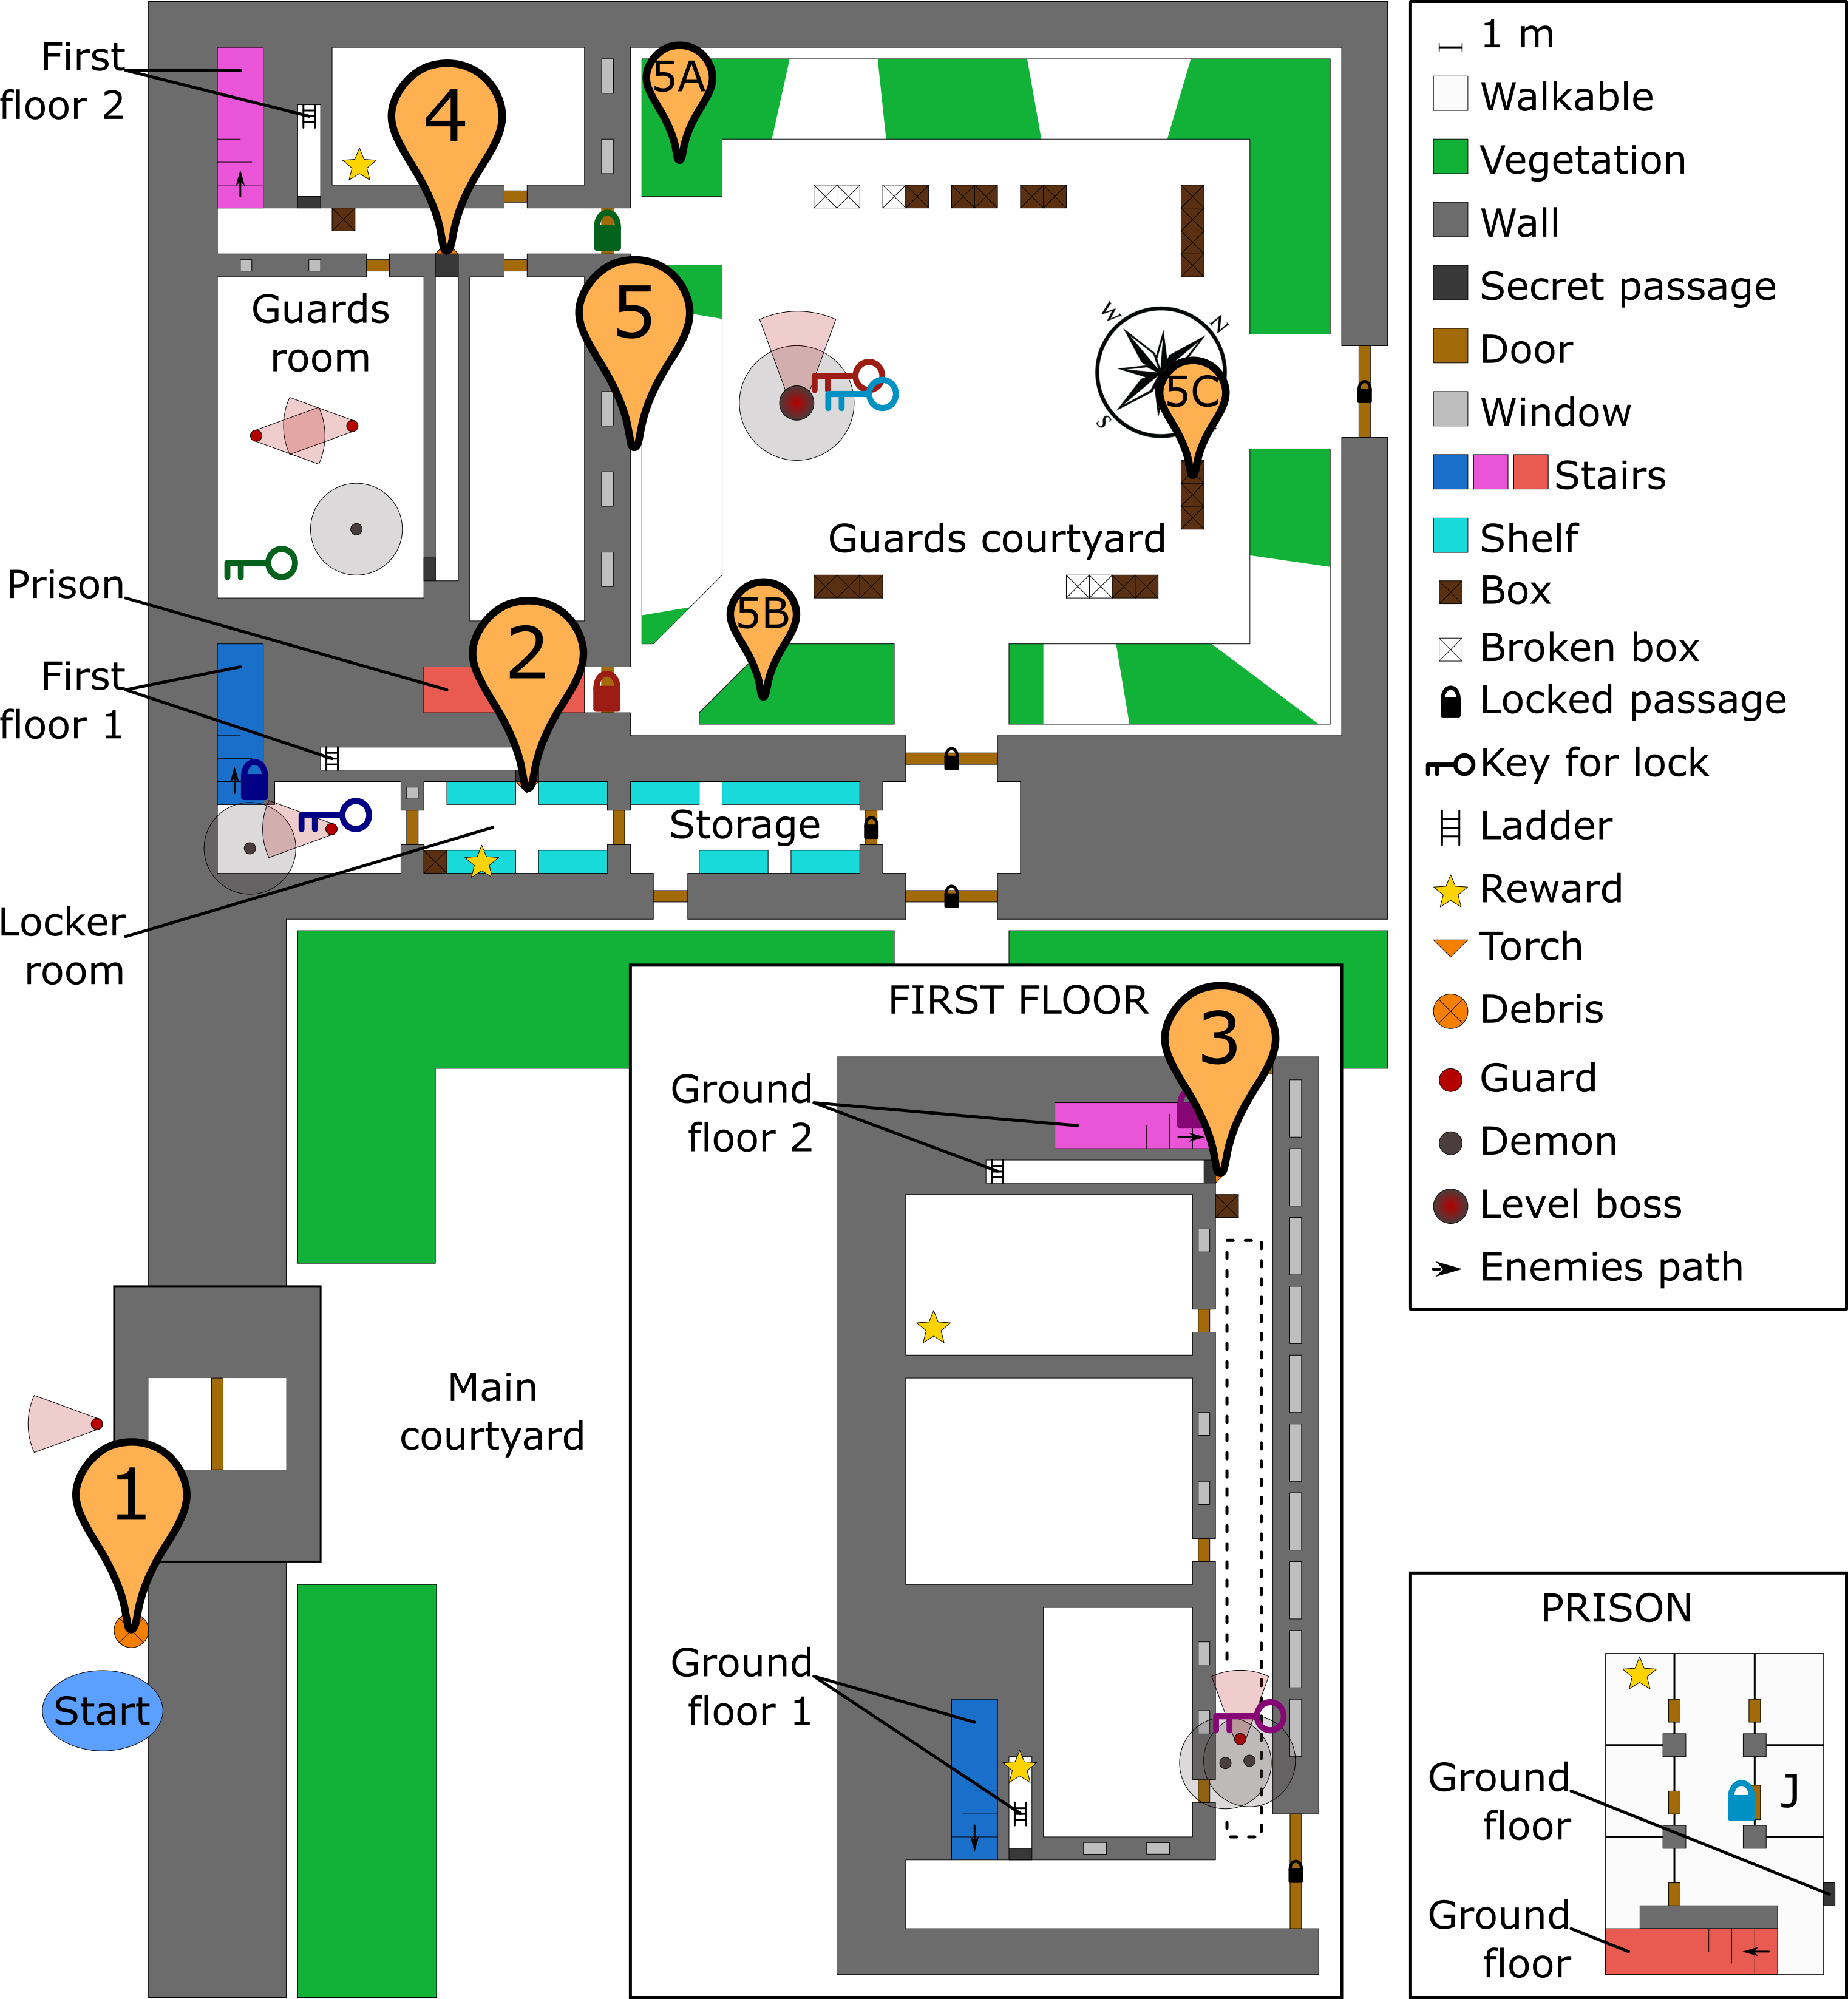
\includegraphics[width=\textwidth]{Images/Maps/castleOfDynamiaPuzzles}
  \caption{Puzzles locations in the Castle of Dynamia}
\end{figure}

\subsection{1. Build a machine}

\begin{figure}[H]
  \centering
  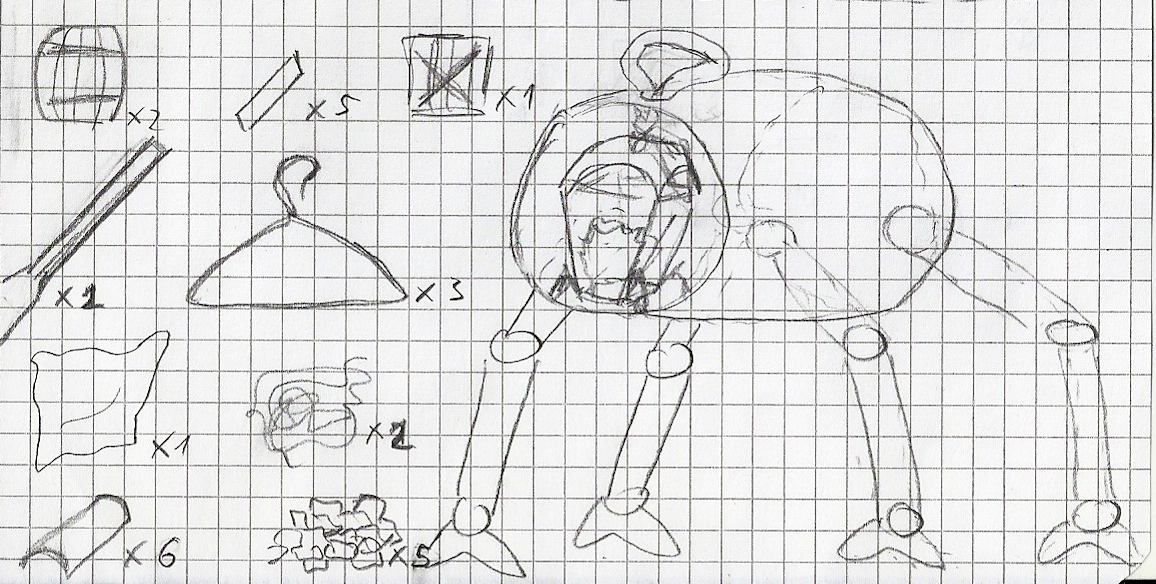
\includegraphics[width=\textwidth]{Images/Puzzles/castleOfDynamia_1}
  \caption{Puzzle 1 in the Castle of Dynamia}
\end{figure}

In order to enter in the courtyard the player can use some debris to build a machine for Calcifer that allows him to climb the wall without being detected.

%The player has different parts and he/she has to understand how to combine them. He/She has to break some part to obtain new components. Some parts are not required to build the machine.

The player has to reorder the pieces of a mosaic representing the machine itself.

The mosaic has 4 rows and 6 columns. The player can switch any couple of two pieces.

\subsubsection*{Hints}
If the player gets stuck for some time, Sophie will tell some lines to help the player, at the same time two pieces will be highlighted in order to suggest to switch them.

\textbf{Sophie}: I think that piece should go there.

\subsection{2. Rotate the torch}

\begin{figure}[H]
  \centering
  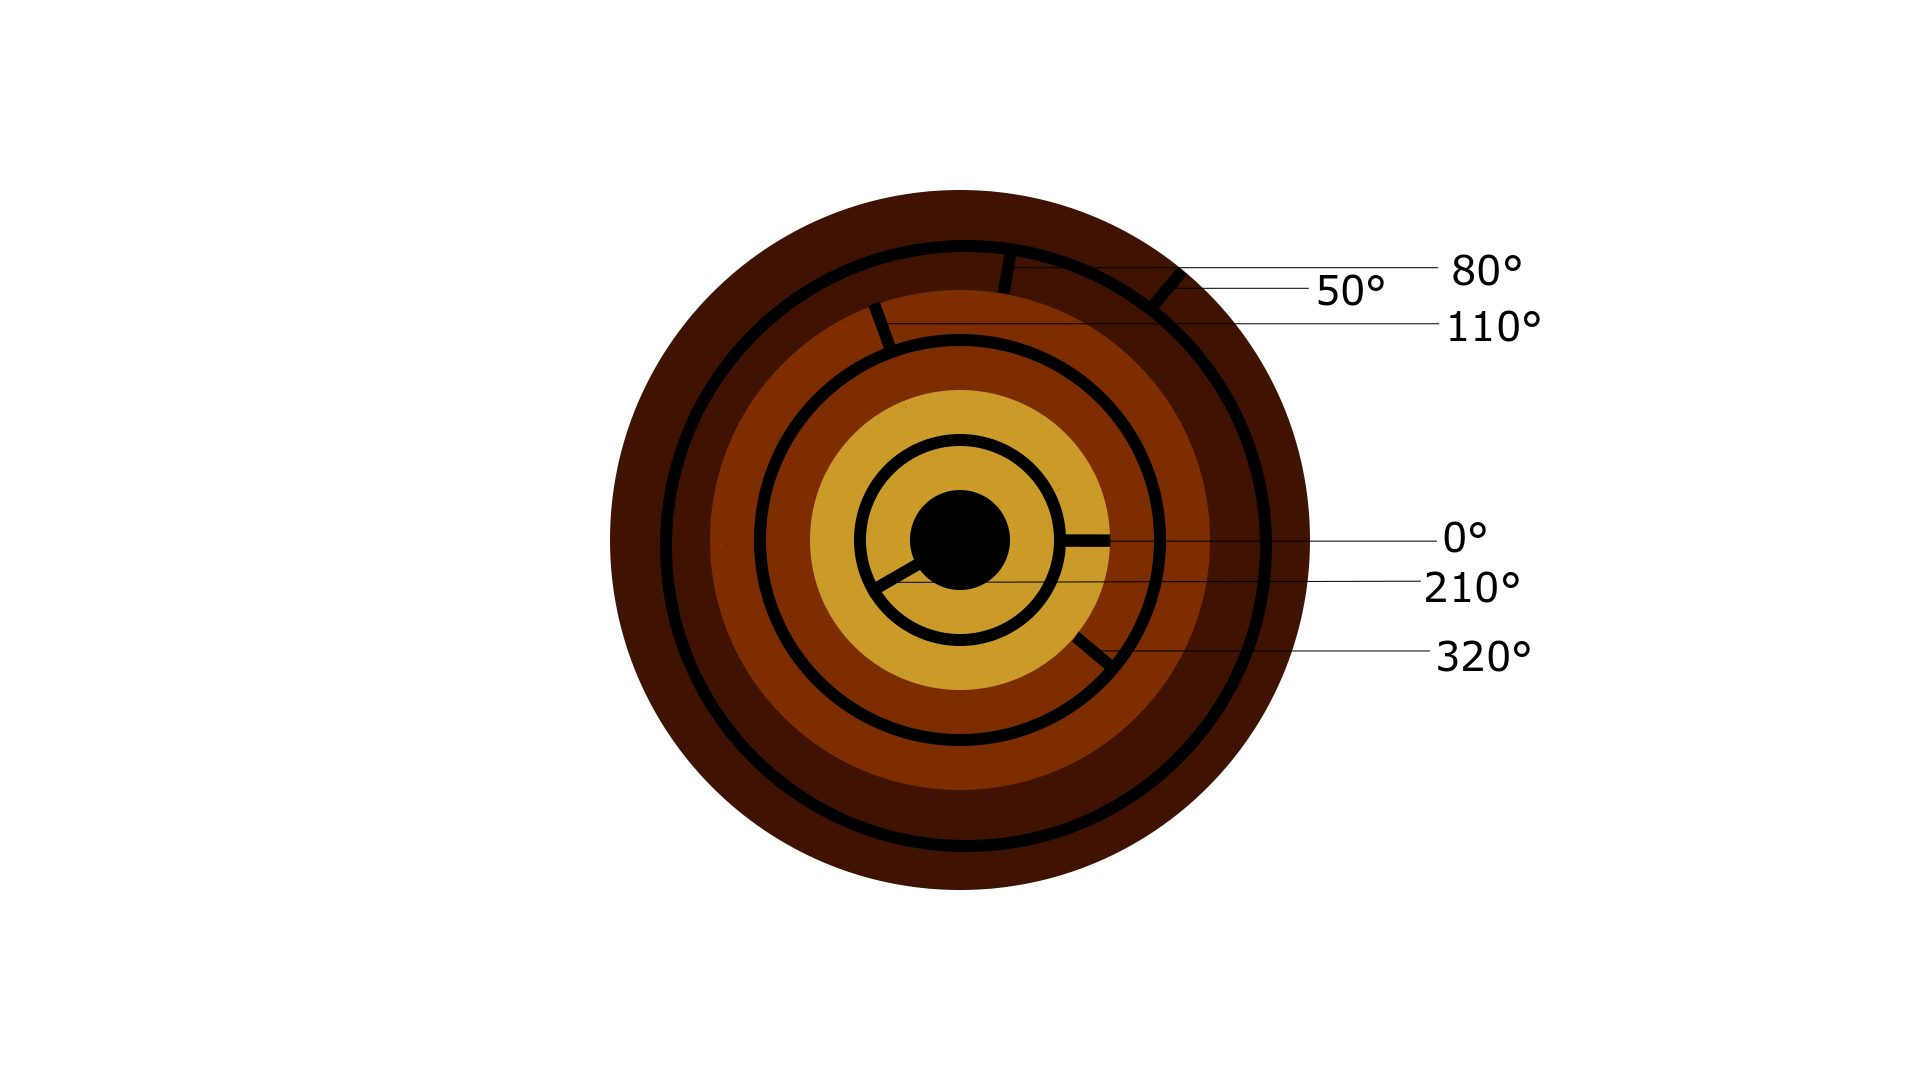
\includegraphics[]{Images/Puzzles/torchPuzzleStart} \quad 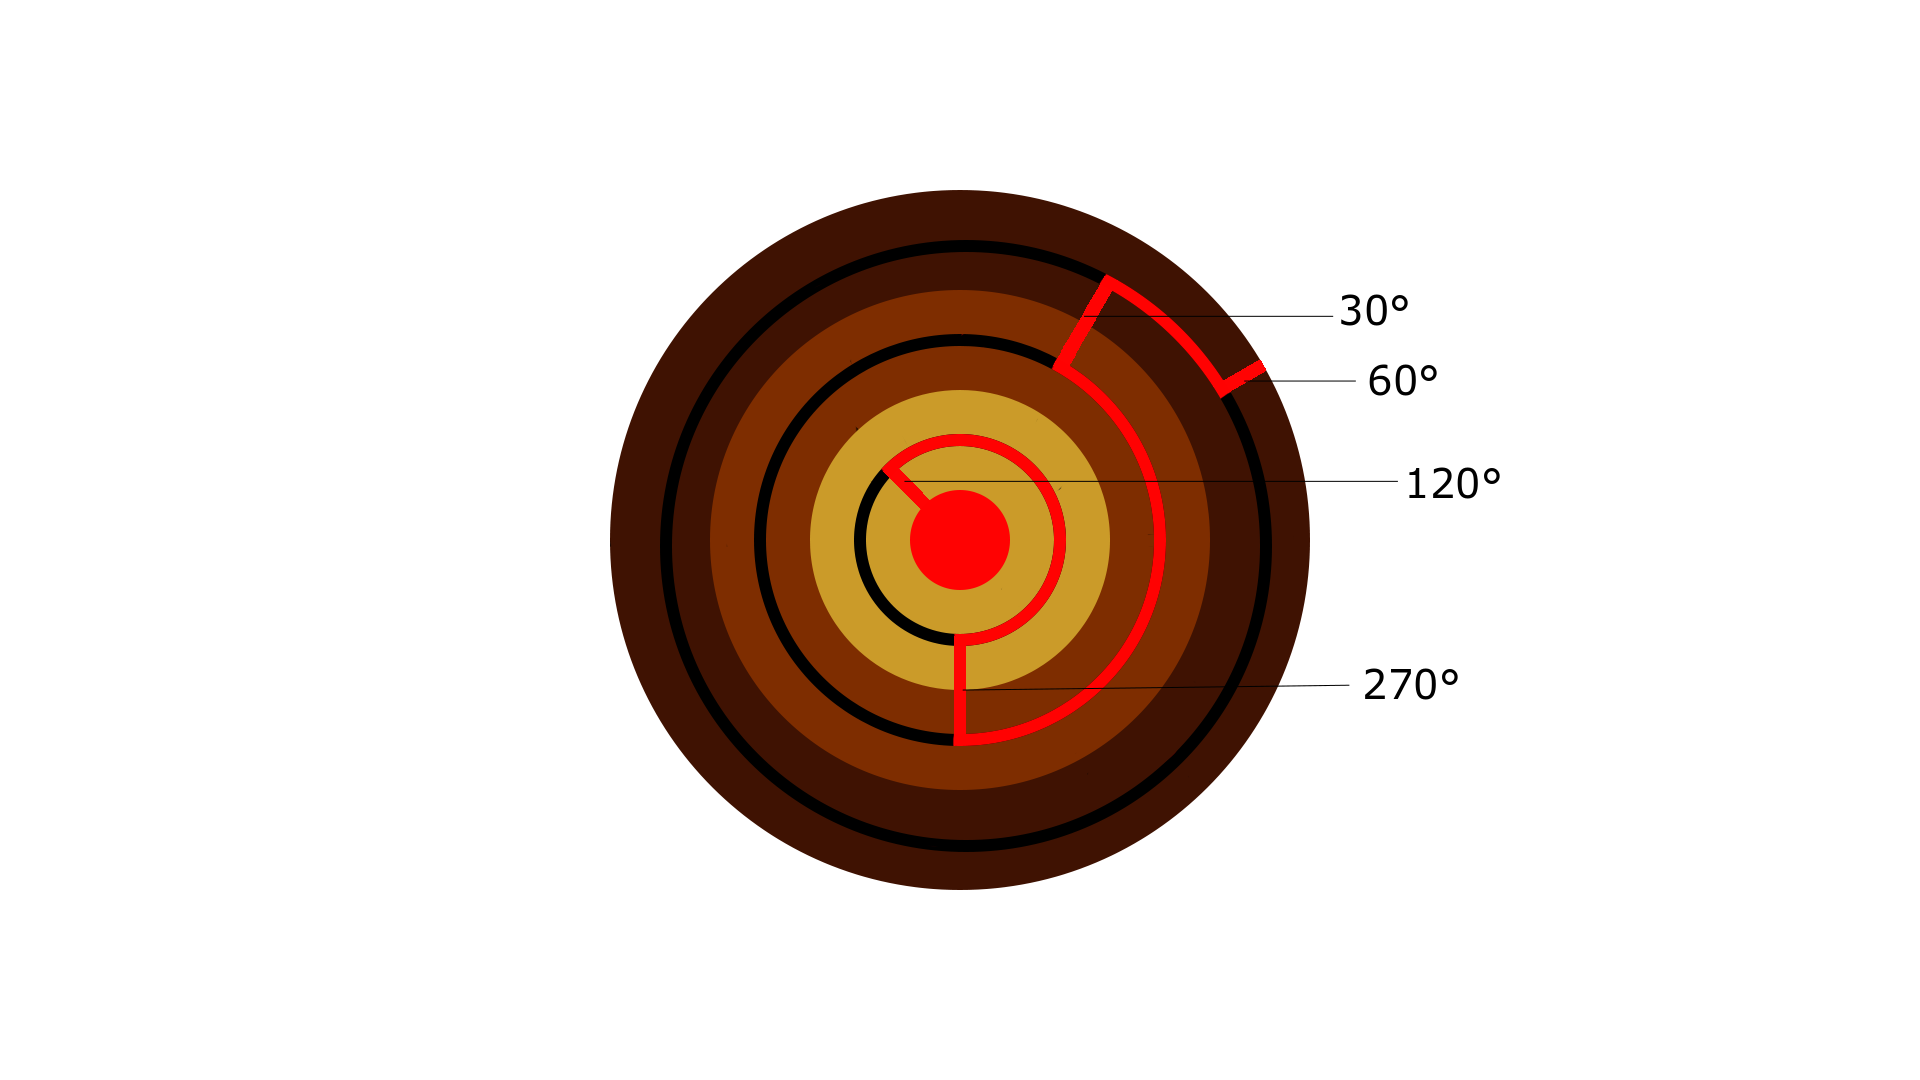
\includegraphics[]{Images/Puzzles/torchPuzzleSolution}
  \caption{Puzzle 2 in the Castle of Dynamia}
\end{figure}

%The torch is a puzzle itself. The player has to rotate the torch and its arms according to the given scheme.

%When the player rotates the main body, the two arms rotate too. When he/she rotates an arm, the main body rotates too, but the other arm stays still.

The player has to rotate three rings on the base of the torch in order to align them in the proper way to create an uninterrupted black path. The player can reset all of the three circles to the starting state by rotating the arm of the torch. The player is supposed to be already taught about how to play this game in the previous levels

When the player rotates the outer ring of one step, the middle ring rotates in the same direction.

When the player rotates the middle ring of one step, the outer ring rotates in the same direction.

When the player rotate the inner ring of one step, the middle ring rotates in the same direction.

\subsubsection*{Technical details}
The starting and the final position of the circles can be found in the pictures here above.

The inner circle rotates by 15 degrees and make the middle one rotate by 15 degrees for each step.

The outer circle rotates by 10 degrees and make the middle one rotate by 5 degrees for each step.

The inner circle rotates by 50 degrees and make the outer one rotate by 15 degrees for each step.


\subsubsection*{Optimal solution}
The solution is composed by three steps (that can be done in any order):

\begin{itemize}
	\item Rotate anticlockwise the inner circle by three steps.
	\item Rotate clockwise the middle circle by two steps.
	\item Rotate clockwise the outer circle by one step.
\end{itemize}

\subsubsection*{Hints}
If the player gets stuck for some time, the torch will tell some lines to help the player.

If the player has not rotated correctly any of the three circle:
\textbf{Torch}: I think turning the rings just randomly is not a good strategy. Try to start again! Rotate my arm!

If the player rotated correctly at least one of the three circles:
\textbf{Torch}: You are on the right track! Keep going!

If the player rotated correctly two of the three circles:
\textbf{Torch}: You are almost done! You are so close!

Once the player has done one of the step of the solution the player will hear a sound feedback: 
\textbf{*CLICK*}

If the player activates the sound feedback but keeps rotating:
\textbf{Torch}:Wait! I have heard something
or
\textbf{Torch} Are you sure? Listen carefully!

\subsection{3. Press the bricks}

\begin{figure}[H]
  \centering
  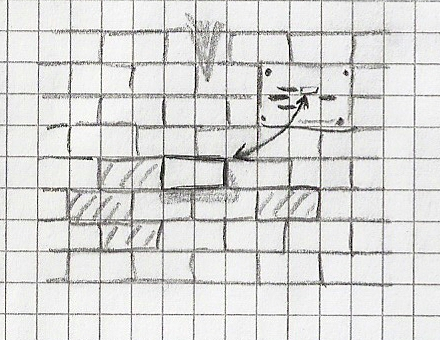
\includegraphics[width=\textwidth]{Images/Puzzles/castleOfDynamia_3}
  \caption{Puzzle 3 in the Castle of Dynamia}
\end{figure}

%Near the torch there is a small plate with some horizontal lines. The player has to press the bricks in the corresponding position under the torch.

%A protruding brick helps the player to identify the bricks to press.

Under the torch there is a small rusty golden plate with four horizontal carved lines, a raised horizontal line and four small arrow

The player has to press the bricks under the torch in the positions corresponding to the carved lines. A protruding brick, corresponding to the raised line, helps the player to identify the bricks to press.

The player has to press the bricks in the order specified by the small arrows.

\subsubsection*{Hints}
If the player gets stuck for some time, the torch will tell some lines to help the player.

\textbf{Torch}: Pss. You have to press the bricks in the proper order. Try to take a closer look to the plate.

\subsection{4. Connect the cables}

\begin{figure}[H]
  \centering
  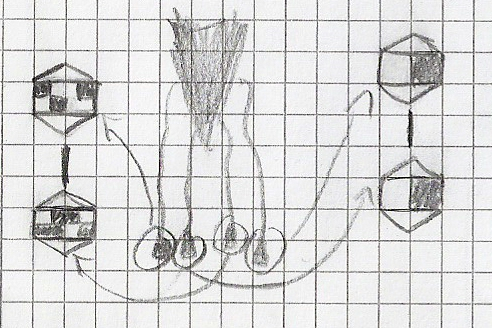
\includegraphics[width=\textwidth]{Images/Puzzles/castleOfDynamia_4}
  \caption{Puzzle 4 in the Castle of Dynamia}
\end{figure}

%There are some cables that hang under the torch. The player has to connect them in the correct pairs, according to the pattern on the plugs.

There are some cables that hang under the torch and two small rusty golden plate, each one with a bars. The bar on the left is full of a red liquid, the other one is empty. Each bar has five marks, one mark per bar is highlighted.

Each cable has a roman number on the plug. The player has to connect the cables on the left with the cables on the right in a way that ensure that the liquid is distributed according to the highlighted marks.

\textit{Example}: I on the left plug and III on the right plug. The liquid will fill 1/4 of the left bar and 3/4 of the right bar.

\subsubsection*{Hints}
If the player gets stuck for some time, the torch will tell some lines to help the player.

\textbf{Torch}: Maths and proportions: young people today don't really study them.
